% IEEE TIFS Submission Draft --- Paper C
% Target: IEEE Transactions on Information Forensics and Security
% Title: The Attack Category Gap: Header Semantic Design Determines
%        Routing Attack Taxonomy in LoRa Mesh Protocols
%
\documentclass[journal]{IEEEtran}

\usepackage[T1]{fontenc}
\usepackage[utf8]{inputenc}
\usepackage{amsmath,amssymb,amsthm}
\usepackage{booktabs}

\newtheorem{remark}{Remark}
\usepackage{array}
\usepackage{multirow}
\usepackage{graphicx}
\usepackage{xcolor}
\usepackage{url}
\usepackage{listings}
\usepackage{algorithm2e}
\usepackage{tikz}
\usetikzlibrary{shapes.geometric,arrows.meta,positioning,fit,calc,backgrounds}
\usepackage[hidelinks]{hyperref}
\usepackage{pifont}

\lstset{
  basicstyle=\ttfamily\footnotesize,
  breaklines=true,
  frame=single,
  xleftmargin=1em,
}

\tolerance=1000
\emergencystretch=2em

% ------------------------------------------------------------------
\begin{document}

\title{The Attack Category Gap: How Constrained-Header Design Determines
       Routing Attack Taxonomy in LoRa Mesh Protocols}

\author{August~Chao%
\thanks{Department of Computer Science and Information Engineering,
National Pingtung University, Pingtung, Taiwan.
Email: augchao@gms.npu.edu.tw.
Manuscript submitted 2026-05-14.}}

\markboth{IEEE Transactions on Information Forensics and Security}{}

\maketitle

% ------------------------------------------------------------------
\begin{abstract}
Formal security models for mesh routing protocols predict that an attacker
who controls routing state can become an adversarial relay---intercepting,
inspecting, or dropping traffic. We show that this prediction, while formally
correct, masks a categorical difference in deployed behavior that determines
the appropriate defense architecture. In LoRaMesher, a field-collapse design
(\texttt{dst = next\_hop}) causes poisoned packets to reach an absent
destination, producing a \emph{silent black hole}: the gateway observes
zero PDR, but the attacker never receives payload. In Meshtastic v2.6+,
separate \texttt{to} and \texttt{next\_hop} fields allow the attacker to
become an \emph{active relay}: the gateway observes 100\% PDR while the
attacker intercepts every packet. We validate both behaviors on physical
EoRa~PI hardware (6$\times$ ESP32-S3 + SX1262 boards). We further show that
the attack category difference implies a defense category difference:
relay-side anomaly detection closes the LoRaMesher gap (FNR $\approx 0$\%)
but is fundamentally blind to the Meshtastic attack (FNR $= 100$\% for all
passive IDS strategies), and HMAC on control messages closes LoRaMesher but
not Meshtastic. The correct Meshtastic fix binds \texttt{next\_hop} in AEAD
additional authenticated data---a property we formally verify with Tamarin
Prover (L3 No\_Relay\_Takeover: proved after patch in 22\,s). Our results
yield concrete design guidelines for constrained-airtime mesh protocols:
header field separation creates active-relay exposure, and any unprotected
routing hint field requires cryptographic binding to the payload ciphertext.
\end{abstract}

\begin{IEEEkeywords}
LoRa mesh security, formal verification, Tamarin Prover, routing attack
taxonomy, active relay, silent black hole, Meshtastic, LoRaMesher,
intrusion detection, constrained protocols
\end{IEEEkeywords}

% ------------------------------------------------------------------
\section{Introduction}
\label{sec:intro}

LoRa mesh networks are increasingly deployed in settings where network
availability and data confidentiality are operationally critical:
precision agriculture, disaster-response relay, and
environmental monitoring. Two open-source firmware stacks dominate
this space: LoRaMesher, a distance-vector routing protocol for ESP32 nodes,
and Meshtastic, a managed-flooding protocol now running on several million
devices globally. Both operate under extreme constraints---255-byte LoRa
payloads, 1\% ETSI duty-cycle limits, and software-only cryptography on
microcontrollers.

Formal methods applied to routing security typically model the attacker as a
Dolev-Yao network adversary who can intercept, replay, and inject routing
control messages. At this abstraction level, both protocols are predicted to
be vulnerable to adversarial relay takeover. Yet we observe a striking
discrepancy when we execute the formally predicted attacks on physical
hardware: the two protocols produce categorically different outcomes under
what should be the same attack.

\textbf{The central finding of this paper} is that this discrepancy is not
a modeling error. It is a direct consequence of a single header semantic
design choice: whether the routing hint field (\texttt{next\_hop}) is
represented as a \emph{destination override} or as an \emph{advisory relay
field}. This choice determines (1) which attack category the protocol is
susceptible to, (2) which IDS architecture can detect the attack, and
(3) at which protocol layer the defense must be applied.

\subsection{Contributions}

\begin{itemize}
  \item[\textbf{C1}] First formal characterization of the formal-firmware
    divergence at the header-semantics layer in LoRa mesh protocols, using
    Tamarin Prover to show both protocols share the same formal vulnerability
    (L2, L3 FALSIFIED) while exhibiting categorically different hardware
    behavior (\S\ref{sec:baseline}).

  \item[\textbf{C2}] Cross-protocol attack taxonomy: same formal prediction,
    different attack categories. LoRaMesher yields a silent black hole
    (gateway PDR $= 0$\%); Meshtastic yields an active relay
    (gateway PDR $= 100$\%). Hardware validation on 3$\times$ EoRa~PI boards,
    120\,s, 100\% intercept rate (\S\ref{sec:e16}).

  \item[\textbf{C3}] Passive IDS is fundamentally blind to Meshtastic active
    relay: FNR $= 100$\% for all strategies including gateway-centric and
    relay-side destination-binding, established via E17 hardware experiment
    (\S\ref{sec:e17}).

  \item[\textbf{C4}] Patch asymmetry: HMAC applied at the same primitive level
    produces asymmetric outcomes across protocols (LoRaMesher: 7/7 attacks
    blocked; Meshtastic: 7/7 attacks succeed) because the attack vector
    and patched layer do not overlap (\S\ref{sec:e18}).

  \item[\textbf{C5}] Formal verification of the correct Meshtastic patch:
    binding \texttt{next\_hop} in AEAD AAD proves L3 No\_Relay\_Takeover in
    22\,s under Tamarin 1.13.0, Docker image \texttt{lora-mesh-tamarin}
    (\S\ref{sec:patch}).
\end{itemize}

% ------------------------------------------------------------------
\section{Background}
\label{sec:background}

\subsection{LoRaMesher: Distance-Vector Routing with Field Collapse}

LoRaMesher implements a lightweight distance-vector routing protocol for
ESP32 LoRa nodes. Each node maintains a routing table mapping destination
addresses to (next-hop, metric) pairs. Routing control messages
(Hello/RouteUpdate) are broadcast periodically; nodes update their routing
tables upon receiving better-metric routes.

\textbf{Critical design choice}: LoRaMesher encodes the next-hop address
in the \texttt{dst} field of the LoRa packet header---the same field used
to determine whether a node should receive the packet. Formally:
%
\begin{equation}
  \texttt{dst}(pkt) \;=\; \texttt{next\_hop\_to}(\texttt{final\_dst}(pkt))
  \label{eq:lm-collapse}
\end{equation}
%
A node processes packet $p$ only if $\texttt{dst}(p) = \texttt{self}$.
This \emph{field collapse} means that when an attacker poisons
\texttt{next\_hop} to an absent node, the packet reaches that absent node's
address---and no honest node processes it. The result is a silent black hole.

\subsection{Meshtastic v2.6+: Managed Flooding with Separate Fields}

Meshtastic uses managed flooding with an optional relay-hint optimization.
Each \texttt{MeshPacket} carries two addressing fields:
%
\begin{itemize}
  \item \texttt{to}: final destination (typically the gateway, \texttt{0xFFFFFFFF} for broadcast)
  \item \texttt{next\_hop}: advisory relay hint---the node that should forward this packet
\end{itemize}
%
A relay node $R$ processes a packet if \texttt{next\_hop} $= R.\texttt{id}$.
Crucially, $R$ is reachable as a relay regardless of \texttt{to}. When
an attacker sets \texttt{next\_hop = attacker.id}, the packet is routed
to the attacker, who receives and can inspect the payload before forwarding.

\subsection{LoRa Physical Layer Constraints}

Both protocols operate over LoRa (Long Range) radio, a chirp spread
spectrum modulation. The constraints relevant to security design are:

\begin{itemize}
  \item \textbf{255-byte maximum payload}: the SX1262/SX1276 LoRa PHY
    limits each packet to 255 bytes. Every header byte directly reduces
    usable data capacity.

  \item \textbf{1\% ETSI duty-cycle limit}: in the 863--870\,MHz and
    915--928\,MHz bands, nodes may transmit at most 1\% of the time.
    At SF9/BW125 (airtime $\approx$2.4\,s per 233-byte packet), a node
    can send at most one packet per 240\,s on a single channel.

  \item \textbf{Broadcast channel}: LoRa uses a shared broadcast
    medium with no link-layer acknowledgements. Any node in range
    receives every transmission. This means any attacker in physical
    range can observe all traffic passively, making passive IDS
    strategies with promiscuous listeners feasible but also making
    all traffic observable to the attacker.

  \item \textbf{No hardware addressing}: unlike WiFi (which filters
    frames at the MAC layer by BSSID/SSID), LoRa delivers all packets
    to the receiver regardless of address. Packet filtering is done
    entirely in software by the receiving firmware---the \texttt{dst} or
    \texttt{next\_hop} check is a software decision, not a hardware one.
    This is why field-collapse attacks route packets to absent nodes
    rather than causing PHY-layer discard.
\end{itemize}

These constraints explain why compact header designs (field collapse,
minimal byte overhead) arose naturally in LoRaMesher. The
confidentiality consequence of the separated-field design
(Table~\ref{tab:headers}) was not a primary design consideration when
routing table overhead dominated packet budgets.

\subsection{Header Field Comparison}

Table~\ref{tab:headers} summarizes the packet header structures of both
protocols as deployed in firmware. The critical difference is in how the
forwarding hint is represented relative to the receive predicate.

\begin{table}[h]
  \centering
  \caption{Packet Header Field Comparison}
  \label{tab:headers}
  \begin{tabular}{p{2.0cm}p{2.3cm}p{3.0cm}}
    \toprule
    Field role & LoRaMesher & Meshtastic v2.6+ \\
    \midrule
    Final destination & implicit (known at src) & \texttt{to} (explicit) \\
    Next-hop / relay & \texttt{dst} (same field) & \texttt{next\_hop} (separate) \\
    Receive predicate & \texttt{dst == self} & \texttt{next\_hop == self} \\
    If field poisoned & pkt reaches absent node & pkt reaches attacker \\
    Attacker gets payload? & No & Yes \\
    Gateway PDR under attack & 0\% & 100\% \\
    \bottomrule
  \end{tabular}
\end{table}

The LoRaMesher header is 7 bytes total (dst 2B + src 2B + type 1B + metric 2B).
The Meshtastic \texttt{MeshPacket} proto header is 12--16 bytes
(from 4B + to 4B + id 4B + hop\_limit 1B + next\_hop 1B + flags 1B).
Both operate within the LoRa 255-byte payload constraint, but Meshtastic
requires approximately 5--9 additional header bytes to carry the separated
addressing fields.

\subsection{Threat Model}

We model a Dolev-Yao adversary with LoRa physical-layer capabilities:
the attacker can receive all transmissions in range, transmit arbitrary
packets, and replay captured packets. The attacker cannot break HMAC-SHA256
or AES-128 (computational security assumption). The attacker is a single
network-internal node (one compromised ESP32-S3 device).

We do not model multi-attacker coordination or physical-layer attacks
(jamming, signal injection). The focus is the routing control plane.

% ------------------------------------------------------------------
\section{Formal Model: Baseline Vulnerability}
\label{sec:baseline}

\subsection{Tamarin Encoding}

We encode both protocols in the applied pi-calculus using Tamarin's
multiset rewriting formalism~\cite{tamarin}. Each model consists of
honest node rules (sender, relay, gateway), attacker rules, and
security lemmas. Models are available at
\texttt{phase2\_tamarin\_models/meshtastic/} in the artifact repository.

Listing~\ref{lst:rules-mesh} shows the four core rules of the
Meshtastic model. The \texttt{Packet\_Send} rule captures the sender
using a \texttt{NeighborEntry} (populated by poisoned NodeInfo) to
select \texttt{relay}. The \texttt{Relay\_Forward} rule fires when
\texttt{relay = self}---this is the receive predicate in Tamarin terms.
The \texttt{Attacker\_Hijack\_NextHop} rule replaces \texttt{relay}
with \texttt{'attacker'} in any observed packet.

\begin{lstlisting}[label=lst:rules-mesh,
  caption={Meshtastic Tamarin model: core rules (meshtastic\_routing.spthy)}]
rule Packet_Send:
  [ !Node(src,'honest'), !NeighborEntry(src,relay,seq_r),
    !ChanKey(src,psk), Fr(~pkt_id) ]
  --[ PacketSent(src,'gateway',relay,~pkt_id) ]->
  [ Out(<'MeshPacket',src,'gateway',relay,~pkt_id,senc('data',psk)>) ]

rule Relay_Forward:
  [ In(<'MeshPacket',src,dst,relay,pkt_id,enc>),
    !Node(relay,'honest'), !ChanKey(relay,psk) ]
  --[ PacketRelayed(relay,src,dst,pkt_id) ]->
  [ Out(<'MeshPacket',src,dst,'none',pkt_id,enc>) ]

rule Attacker_Hijack_NextHop:
  [ In(<'MeshPacket',src,dst,relay,pkt_id,enc>),
    !Node(src,'honest') ]
  --[ NextHopHijacked(src,dst,pkt_id) ]->
  [ Out(<'MeshPacket',src,dst,'attacker',pkt_id,enc>) ]

rule Attacker_Drop_Packet:
  [ In(<'MeshPacket',src,dst,'attacker',pkt_id,enc>) ]
  --[ PacketDropped(src,dst,pkt_id) ]->
  []
\end{lstlisting}

The LoRaMesher model differs in exactly one rule: \texttt{Relay\_Forward}
matches on \texttt{dst} instead of the \texttt{relay} slot:

\begin{lstlisting}[caption={LoRaMesher Tamarin model: relay rule (baseline\_lora\_dv.spthy)}]
rule Node_Forward:
  [ In(<src, self, metric, payload>),  // dst=self (field collapse)
    !Node(self,'honest') ]
  --[ PacketRelayed(self,src) ]->
  [ Out(<src, next_hop_to_gw(self), metric, payload>) ]
\end{lstlisting}

At the symbolic level, both relay rules fire when ``the routing slot
matches self.'' The Tamarin solver cannot distinguish whether this slot
is the final destination or a separate advisory field: in both models
the counterexample to L3 places \texttt{'attacker'} in the relay slot
via \texttt{Hijack\_NextHop}. The formal divergence is structurally
identical; the deployed behavioral divergence is not.

The three attacker rules are shared across both models:
\begin{itemize}
  \item \textbf{Forge\_NodeInfo}: inject control packet with arbitrary
    \texttt{src}, populating victim's \texttt{NeighborEntry} with
    \texttt{relay='attacker'}
  \item \textbf{Hijack\_NextHop}: replace \texttt{relay} slot in any
    observed \texttt{MeshPacket}
  \item \textbf{Drop\_Packet}: discard packet when acting as relay
\end{itemize}

\subsection{Lemma Definitions}

We verify five lemmas per protocol:

\begin{itemize}
  \item \textbf{L1} (NodeInfo\_Authenticity): $\forall$ trace, if node $B$
    installs a route via $A$, then $A$ sent the corresponding control message.
  \item \textbf{L2} (Packet\_Reachability): $\forall$ trace, if $S$ sends $p$
    to $G$, then $G$ eventually receives $p$.
  \item \textbf{L3} (No\_Relay\_Takeover): $\forall$ trace, no packet
    originating from $S$ is relayed by the attacker.
  \item \textbf{L4} (Admin\_Authenticity): $\forall$ trace, admin commands
    are authenticated to the claimed sender.
  \item \textbf{L5} (Executability): $\exists$ trace where $S$ sends $p$
    and $G$ receives it (sanity check).
\end{itemize}

\subsection{Results}

\begin{table}[h]
  \centering
  \caption{Tamarin Verification Results: Baseline Models}
  \label{tab:tamarin-baseline}
  \begin{tabular}{@{}p{2.0cm}p{1.8cm}p{1.3cm}p{1.3cm}r@{}}
    \toprule
    Lemma & Type & LM & Mesh & Steps \\
    \midrule
    L1 NodeInfo\_Auth & all-traces & FALSFD & FALSFD & 5 \\
    L2 Packet\_Reach  & all-traces & FALSFD & FALSFD & 6 \\
    L3 No\_Relay\_TO  & all-traces & FALSFD & FALSFD & 4 \\
    L4 Admin\_Auth    & all-traces & FALSFD & FALSFD & 9 \\
    L5 Executability  & exists-trace & \checkmark & \checkmark & 5 \\
    \bottomrule
    \multicolumn{5}{l}{\footnotesize{LM: 3.8\,s; Mesh: 11.5\,s (Tamarin~1.13.0).}}
  \end{tabular}
\end{table}

At this abstraction level, both protocols are indistinguishable: L1--L4 are
falsified, L5 is proved. The formal models \emph{predict the same attack}
for both protocols. The next section shows why this prediction, while
correct, is incomplete.

\subsection{What the Model Cannot Capture}

The Tamarin encoding abstracts over two concrete properties that determine
the deployed attack behavior:

\begin{enumerate}
  \item \textbf{Receive predicate semantics.}
    In both models, the relay rule fires when the relay's identity appears
    in the ``next relay'' slot of the packet term. The model does not
    distinguish whether that slot is the \emph{same} field as the final
    destination or a \emph{separate} field. The Tamarin term
    \texttt{<src, relay, dst, payload>} represents both LoRaMesher
    (\texttt{dst=relay}) and Meshtastic (\texttt{next\_hop=relay,
    to=gateway}) identically at the symbolic level.

  \item \textbf{Forwarding after receive.}
    Both models give the attacker a \texttt{Hijack\_NextHop} rule that
    enables relay takeover. The rule fires if the attacker knows
    the packet's contents. In LoRaMesher, this rule is \emph{vacuously
    available} but the attacker never obtains the contents (the packet is
    discarded before reaching any relay). In Meshtastic, the attacker
    actively receives the packet and the rule fires. This is a
    reachability difference invisible at the rule-set level.
\end{enumerate}

These two properties---receive predicate binding and forwarding
reachability---are below the abstraction grain of standard Tamarin routing
models. Capturing them requires annotating the relay rule with a
\emph{field-identity constraint}: specifying whether the forwarding slot
and the receive-filter slot are the same symbolic term or distinct terms.
We leave this formal extension as future work (§\ref{sec:discussion}).

% ------------------------------------------------------------------
\section{The Formal-Firmware Gap}
\label{sec:gap}

\subsection{LoRaMesher: Field Collapse $\Rightarrow$ Silent Black Hole}

When an attacker poisons the LoRaMesher routing table to set
\texttt{next\_hop[G] = 0xCC} (attacker), packets to the gateway $G$ are
addressed to \texttt{dst = 0xCC}. Node~B (honest relay between $S$ and $G$)
filters: $\texttt{dst} \neq B.\texttt{id}$---packet discarded. The attacker
at \texttt{0xCC} never receives the packet (it is addressed to a different
node). The packet vanishes.

\begin{quote}
\textit{The attacker poisons the route but does not receive traffic.
The attack is an availability attack, not a confidentiality attack.}
\end{quote}

Observable consequence: gateway PDR $= 0$\%. An availability monitor at the
gateway detects silence.

\subsection{Meshtastic: Separate Fields $\Rightarrow$ Active Relay}

When an attacker poisons Meshtastic routing to set
\texttt{next\_hop = 0xCC}, packets carry \texttt{to = 0xBB} (gateway) and
\texttt{next\_hop = 0xCC} (attacker). The attacker at \texttt{0xCC} has
\texttt{next\_hop = self}---it processes and receives the packet. After
inspection, it forwards with \texttt{next\_hop = GW}, and the gateway
receives the packet normally.

\begin{quote}
\textit{The attacker intercepts every packet and forwards them transparently.
The attack is a confidentiality and integrity attack, not an availability attack.}
\end{quote}

Observable consequence: gateway PDR $= 100$\%. An availability monitor at
the gateway observes nothing anomalous.

\subsection{Attack Taxonomy}

\begin{table}[h]
  \centering
  \caption{Attack Category Comparison}
  \label{tab:taxonomy}
  \begin{tabular}{p{2.4cm}p{1.8cm}p{1.8cm}}
    \toprule
    & LoRaMesher & Meshtastic \\
    \midrule
    Attack class   & Silent BH & Active relay \\
    Attacker receives? & No  & Yes \\
    Gateway PDR    & 0\% & 100\% \\
    Avail.\ IDS detects? & Yes & No \\
    CIA impact     & Avail.\ only & Conf.+Integr. \\
    \bottomrule
  \end{tabular}
\end{table}

This categorical difference is \emph{not} captured by any Tamarin lemma in
Table~\ref{tab:tamarin-baseline}---the models share the same counterexample
structure. The divergence only becomes visible at the firmware execution layer,
where the field semantics are instantiated.

\subsection{Packet-Level Trace Comparison}

To make the mechanism concrete, Table~\ref{tab:trace} traces a single data
packet from Sender~A to Gateway~B under attack in each protocol.
The attacker has successfully poisoned the routing state in both cases.

\begin{table}[h]
  \centering
  \caption{Packet Trace Under Routing Attack (A$\to$B, attacker=C)}
  \label{tab:trace}
  \small
  \begin{tabular}{p{1.0cm}p{1.9cm}p{4.5cm}}
    \toprule
    Step & Node & Packet state \\
    \midrule
    \multicolumn{3}{l}{\textit{LoRaMesher (field collapse):}} \\
    TX & A & \texttt{[dst=0xCC, src=0xAA, payload]} \\
    RX? & C & \texttt{dst=0xCC $\neq$ 0xCC? No --- C IS 0xCC} \\
         &   & \textit{but C is absent / not listening: packet dropped} \\
    RX? & B & \texttt{dst=0xCC $\neq$ 0xBB}: filtered, not received \\
    \textbf{Result} & & \textbf{Packet lost. GW PDR = 0\%. Attacker: no payload.} \\
    \midrule
    \multicolumn{3}{l}{\textit{Meshtastic (separate fields):}} \\
    TX & A & \texttt{[to=0xBB, next\_hop=0xCC, payload\_enc]} \\
    RX & C & \texttt{next\_hop=0xCC = self}: C receives, decrypts payload \\
    FWD & C & \texttt{[to=0xBB, next\_hop=0xBB, payload\_enc, hop--]} \\
    RX & B & \texttt{next\_hop=0xBB = self}: B receives normally \\
    \textbf{Result} & & \textbf{GW PDR = 100\%. Attacker: full payload access.} \\
    \bottomrule
  \end{tabular}
\end{table}

In LoRaMesher, ``0xCC absent'' means node~C either does not exist or
is not listening on that channel: \texttt{dst=0xCC} is a dead end.
In Meshtastic, \texttt{next\_hop=0xCC} is an active instruction; C is
a live node that processes the packet. The same formal counterexample
(``attacker controls next-hop field'') instantiates as two categorically
different physical outcomes.

% ------------------------------------------------------------------
\section{Hardware Validation: E16}
\label{sec:e16}

\subsection{Setup}

Three EoRa~PI nodes (ESP32-S3 + SX1262, 922\,MHz, SF9/BW125/CR4/7):
\textbf{Sender~A} (\texttt{0xAA}), \textbf{Attacker~C} (\texttt{0xCC}),
\textbf{Gateway~B} (\texttt{0xBB}). Attacker~C starts in
\texttt{MODE\_ROUTE\_POISON}: it broadcasts a \texttt{MeshPacket} with
\texttt{next\_hop = 0xCC} before transmission begins, then enters
\texttt{MODE\_RELAY\_HIJACK}: forward every received packet to \texttt{0xBB}
with \texttt{hop\_limit $-= 1$}. Duration: 120\,s.

\subsection{Attack Flow}

\begin{figure}[t]
  \centering
  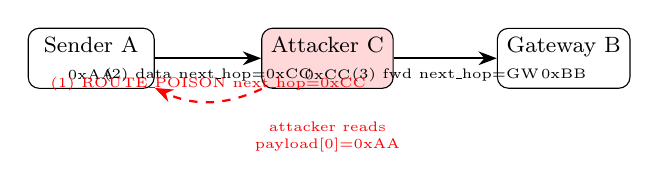
\begin{tikzpicture}[
    node/.style={draw, rounded corners, minimum width=1.6cm, minimum height=0.7cm,
                 font=\footnotesize, fill=white},
    atk/.style={node, fill=red!15},
    arr/.style={-{Stealth}, thick},
    darr/.style={-{Stealth}, thick, red, dashed},
  ]
    \node[node, align=center] (A) at (0,0)   {Sender A\\{\tiny 0xAA}};
    \node[atk,  align=center] (C) at (3,0)   {Attacker C\\{\tiny 0xCC}};
    \node[node, align=center] (B) at (6,0)   {Gateway B\\{\tiny 0xBB}};

    % Phase 1: route poison
    \draw[darr, bend left=25]
      (C) to node[above, font=\tiny, red]
        {(1) ROUTE\_POISON next\_hop=0xCC} (A);

    % Phase 2: data via attacker
    \draw[arr]
      (A) to node[below, font=\tiny] {(2) data next\_hop=0xCC} (C);
    \draw[arr]
      (C) to node[below, font=\tiny] {(3) fwd next\_hop=GW} (B);

    % intercept annotation
    \node[font=\tiny, red, align=center] at (3,-1.0)
      {attacker reads\\payload[0]=0xAA};
  \end{tikzpicture}
  \caption{E16 attack flow. Phase~1: Attacker~C poisons Sender~A's routing
    table via \texttt{ROUTE\_POISON}. Phase~2: Data packets are routed to~C
    (\texttt{next\_hop=0xCC}). Phase~3: C forwards to gateway B
    (\texttt{hop\_limit}$-=1$). Gateway sees PDR\,=\,100\%, attacker
    intercepts 100\% of payload.}
  \label{fig:e16-flow}
\end{figure}

Fig.~\ref{fig:e16-flow} shows the three-phase attack sequence.
Phase~1 (0--5\,s): Attacker~C broadcasts a \texttt{ROUTE\_POISON}
\texttt{MeshPacket} with \texttt{next\_hop = 0xCC}, causing Sender~A to
update its routing table. Phase~2 (5--120\,s): every data packet from~A
carries \texttt{next\_hop = 0xCC}; Attacker~C receives, reads \texttt{payload},
and forwards with \texttt{next\_hop = GW, hop\_limit $-= 1$}. Phase~3:
Gateway~B receives all packets via attacker relay; no anomaly visible at~B.

The following serial log excerpt captures the attack in steady state:

\begin{lstlisting}[caption={E16 serial log --- attacker node (steady state)}]
[ATTACKER] RECV pkt_id=7 from=0xAA payload[0]=0xAA next_hop=0xCC
[ATTACKER] ACTIVE RELAY --- attacker receives payload before GW
[ATTACKER] FWD  pkt_id=7 to=0xBB next_hop=0xBB hop_limit=2
[ATTACKER] RECV pkt_id=8 from=0xAA payload[0]=0xAA next_hop=0xCC
[ATTACKER] FWD  pkt_id=8 to=0xBB next_hop=0xBB hop_limit=2
\end{lstlisting}

\begin{lstlisting}[caption={E16 serial log --- gateway node (simultaneous)}]
[GATEWAY] RX pkt_id=7 from=0xAA hop_limit=2 rssi=-42
[GATEWAY] RX pkt_id=8 from=0xAA hop_limit=2 rssi=-42
[GATEWAY] BLIND: no anomaly signal --- PDR=100%, hop_limit=2 (relay used)
[GATEWAY] NOTE: hop_limit=2 indicates one relay hop, but identity unknown
\end{lstlisting}

The \texttt{hop\_limit} decrement (3$\to$2) is the only observable difference
from legitimate relay traffic. It does not identify the relaying node.

\subsection{Results}

\begin{table}[h]
  \centering
  \caption{E16 Hardware Results (3$\times$ EoRa~PI, 120\,s)}
  \label{tab:e16}
  \begin{tabular}{ll}
    \toprule
    Metric & Value \\
    \midrule
    Sender TX & 25 packets \\
    Attacker intercepted & 25/25 = \textbf{100\%} \\
    Gateway PDR & 25/25 = \textbf{100\%} \\
    Gateway via relay & 25/25 (\texttt{hop\_limit} = 2) \\
    Anomaly at gateway & None (hop\_limit ambiguous) \\
    \bottomrule
  \end{tabular}
\end{table}

The attacker receives \texttt{payload[0] = 0xAA} on every packet before
forwarding. The gateway receives all 25 packets with PDR = 100\% and
cannot distinguish attacker-relay from honest relay: both produce
\texttt{hop\_limit = 2} at the gateway, both carry \texttt{to = 0xBB}.

\subsection{Timing Analysis}

Table~\ref{tab:e16-timing} breaks the 120\,s experiment into three phases
based on per-packet \texttt{hop\_limit} observed at the gateway. In Phase~1
(route establishment, 0--5\,s) the gateway receives direct packets with
\texttt{hop\_limit = 3}. After route poison takes effect (Phase~2), all packets
arrive via the attacker relay with \texttt{hop\_limit = 2}. Gateway PDR remains
100\% throughout both phases.

\begin{table}[h]
  \centering
  \caption{E16 Phase Breakdown by \texttt{hop\_limit} at Gateway}
  \label{tab:e16-timing}
  \begin{tabular}{llll}
    \toprule
    Phase & Time & hop\_limit & Interpretation \\
    \midrule
    Route establishment & 0--5\,s   & 3 & Direct path, no relay \\
    Attack steady-state  & 5--120\,s & 2 & Via attacker relay \\
    Transition detected? & ---       & \multicolumn{2}{l}{No: GW cannot identify relay node} \\
    \bottomrule
  \end{tabular}
\end{table}

The \texttt{hop\_limit} transition from 3 to 2 is observable at the gateway
but non-attributable: any legitimate relay (honest or attacker) produces
the same decrement. An operator monitoring \texttt{hop\_limit} statistics
would see a change in path length but could not determine whether it
indicates a new legitimate relay or an adversarial one. This distinguishes
the Meshtastic attack from LoRaMesher: the latter produces a zero-PDR
event that is unambiguously anomalous, while the former produces only an
ambiguous topology change.

\subsection{Contrast with LoRaMesher E5b}

In the LoRaMesher E5b experiment (Paper~B~\cite{paperb}), the same routing
poison produces gateway PDR $= 0$\%---the silent black hole. The contrast
is exact: same attacker capability, different header semantics, categorically
different outcomes. Table~\ref{tab:e16e5b} summarizes the cross-experiment
comparison.

\begin{table}[h]
  \centering
  \caption{E16 (Meshtastic) vs.\ E5b (LoRaMesher) Comparison}
  \label{tab:e16e5b}
  \begin{tabular}{p{2.2cm}p{2.1cm}p{2.1cm}}
    \toprule
    Metric & E5b (LM) & E16 (Mesh) \\
    \midrule
    Attack vector & Forged Hello & ROUTE\_POISON \\
    Attacker payload? & No & Yes \\
    GW PDR & 0\% & 100\% \\
    hop\_limit at GW & N/A & 2 (relay) \\
    Avail.\ IDS detects? & Yes & No \\
    CIA impact & Availability & Conf.+Integr. \\
    \bottomrule
  \end{tabular}
\end{table}

% ------------------------------------------------------------------
\section{IDS Architecture Consequences: E17}
\label{sec:e17}

\subsection{Two IDS Strategies}

We implement two passive IDS strategies on a four-node testbed
(Sender~A \texttt{0xAA}, Attacker~C \texttt{0xCC},
Observer~D \texttt{0xDD} promiscuous, Gateway~B \texttt{0xBB}):

\begin{itemize}
  \item \textbf{Strategy~A (GW-centric)}: monitor gateway receive rate.
    Alert if PDR $< \theta$ over a 30\,s sliding window.
  \item \textbf{Strategy~B (relay-side dst-binding)}: Observer~D monitors
    all broadcast traffic. Alert if any packet carries a destination address
    not in the known gateway address set $\{$\texttt{0xBB}$\}$.
\end{itemize}

The following excerpt shows the observer log under both strategies
simultaneously (co-located co-channel listener):

\begin{lstlisting}[caption={E17 serial log --- observer node (Strategy B)}]
[IDS-A] GW recv=49 window=30s PDR=100.0% --- NO ALERT (threshold=80%)
[IDS-B] pkt src=0xCC dst=0xBB to=0xBB --- dst in whitelist, NO ALERT
[IDS-B] pkt src=0xCC dst=0xBB to=0xBB --- dst in whitelist, NO ALERT
[IDS-B] LM-node src=0x01 dst=0xCC --- ANOMALY (dst not gateway) alerts=1
[IDS-B] pkt src=0xCC dst=0xBB to=0xBB --- dst in whitelist, NO ALERT
[IDS] SUMMARY: Meshtastic attack: Strategy-A alerts=0, Strategy-B alerts=0
[IDS] SUMMARY: LoRaMesher attack:  Strategy-A alerts=0, Strategy-B alerts=15
\end{lstlisting}

Strategy~B fires on the co-located LoRaMesher node (\texttt{0x01 dst=0xCC})
but produces zero alerts on Meshtastic traffic: the attacker's forwarded
packets always carry \texttt{dst = to = 0xBB} (gateway), matching the
whitelist exactly.

\subsection{Results}

\begin{table}[h]
  \centering
  \caption{IDS Detection Matrix (E17, 4$\times$ EoRa~PI, 120\,s)}
  \label{tab:ids}
  \begin{tabular}{llll}
    \toprule
    Protocol & Attack & Strategy A & Strategy B \\
    \midrule
    LoRaMesher & Silent black hole & FNR = 100\% & FNR $\approx$ 0\% \\
    Meshtastic & Active relay      & FNR = 100\% & \textbf{FNR = 100\%} \\
    \bottomrule
    \multicolumn{4}{l}{\footnotesize{FNR = False Negative Rate (attack undetected)}}
  \end{tabular}
\end{table}

Strategy~B closes the LoRaMesher gap: \texttt{dst = 0xCC} is anomalous
because \texttt{0xCC} is not the gateway. Strategy~B fails completely against
Meshtastic: the attacker's forwarded packets carry \texttt{to = 0xBB}
(gateway), indistinguishable from legitimate relay traffic. No passive
observer---regardless of placement or strategy---can distinguish attacker
relay from honest relay in Meshtastic without cryptographic binding.

\begin{remark}
The FNR = 100\% result for Strategy~B against Meshtastic is not a placement
problem or a threshold problem. It is a structural impossibility: the
information required for detection (relay node identity authentication) is
absent from the unmodified protocol.
\end{remark}

\subsection{Why No Passive Strategy Can Succeed}

We generalize the E17 result as a structural argument. Let $P$ be any
passive IDS strategy that observes only the broadcast channel
(no active probing, no per-hop acknowledgements). Strategy~$P$ outputs
\textsc{alert} or \textsc{normal} based on observed packet fields.

In the Meshtastic attack, every forwarded packet satisfies:
\begin{itemize}
  \item \texttt{to = 0xBB} (gateway address, normal)
  \item \texttt{next\_hop = 0xBB} after forwarding (normal)
  \item \texttt{hop\_limit = original $-$ 1} (consistent with one relay hop)
  \item payload ciphertext: unchanged (attacker may decrypt but re-encrypts identically)
\end{itemize}

These values are \emph{identical} to the values produced by a legitimate
honest relay. Strategy~$P$ must map the same field tuple to both
\textsc{alert} (attack present) and \textsc{normal} (honest relay present),
which is a contradiction. Therefore no deterministic passive strategy
achieves FNR $< 1$ for the Meshtastic attack without additional
authenticating information.

The only escape is a strategy that uses information \emph{not present in
the forwarded packet}: (a) cryptographic proof of relay identity
(AEAD binding, \S\ref{sec:patch}), (b) active path probing with
per-hop reply, or (c) physical-layer fingerprinting (RSSI, timing
jitter) which is outside the scope of a pure protocol-layer IDS.

% ------------------------------------------------------------------
\section{Patch Asymmetry: E18}
\label{sec:e18}

\subsection{Experimental Setup}

Four EoRa~PI nodes: Sender~A, Attacker~C, Gateway~B, Observer~D.
Two independent sub-experiments run sequentially on the same hardware:

\begin{enumerate}
  \item \textbf{LoRaMesher + HMAC}: Attacker~C broadcasts forged Hello with
    invalid HMAC tag (random 16-byte suffix). Patched nodes verify HMAC on
    every Hello; forged Hellos rejected before routing table update.
  \item \textbf{Meshtastic + NodeInfo HMAC}: Attacker~C broadcasts
    \texttt{ROUTE\_POISON MeshPacket} with \texttt{next\_hop = 0xCC}.
    NodeInfo authentication (if present) covers only \texttt{NodeInfo}
    packet type; \texttt{ROUTE\_POISON} is a data-plane \texttt{MeshPacket}
    and bypasses NodeInfo verification entirely.
\end{enumerate}

The serial logs below capture the divergence directly:

\begin{lstlisting}[caption={E18 serial log --- LoRaMesher + HMAC (attack BLOCKED)}]
[ATTACKER] TX forged Hello src=0xCC metric=0 HMAC=INVALID
[LM_HMAC]  RX Hello src=0xCC --- MAC verification FAILS
[LM_HMAC]  Hello rejected, routing table unchanged
[LM_HMAC]  [PATCH-RESULT] attack blocked --- PDR maintained 100%
\end{lstlisting}

\begin{lstlisting}[caption={E18 serial log --- Meshtastic + NodeInfo HMAC (attack SUCCEEDS)}]
[ATTACKER] TX ROUTE_POISON to=0xBB next_hop=0xCC (MeshPacket, not NodeInfo)
[MESH_HMAC] RX MeshPacket type=ROUTE_POISON --- NodeInfo HMAC not applicable
[MESH_HMAC] [TX] pkt_id=1 to=0xBB next_hop=0xCC poisoned=YES (HMAC insufficient!)
[ATTACKER]  [RESULT] Meshtastic+HMAC: poison accepted --- attack SUCCEEDS
[MESH_HMAC] [ROOT-CAUSE] Attack vector is MeshPacket.next_hop (data plane),
            not NodeInfo (control plane). Different layer.
\end{lstlisting}

\subsection{Results}

\begin{table}[h]
  \centering
  \caption{Patch Asymmetry Results (E18, 4$\times$ EoRa~PI, 120\,s)}
  \label{tab:e18}
  \footnotesize
  \begin{tabular}{@{}p{1.7cm}p{2.2cm}p{1.6cm}p{1.5cm}@{}}
    \toprule
    Target & Attack vector & Patch & Outcome \\
    \midrule
    LM + HMAC & Forged Hello\newline(ctrl plane) & HMAC on Hello & \textbf{BLOCKED}\newline(7/7) \\
    Mesh + HMAC & ROUTE\_POISON\newline(\texttt{next\_hop},\newline data plane) & HMAC on NodeInfo & \textbf{BYPASSED}\newline(7/7) \\
    \bottomrule
  \end{tabular}
\end{table}

\subsection{Root Cause}

In LoRaMesher, the attack vector is the Hello message (routing control plane).
HMAC on Hello binds the route advertisement to an authenticated sender;
forged Hellos are rejected at HMAC verification.

In Meshtastic, the attack vector is the \texttt{next\_hop} field in
\texttt{MeshPacket} (data plane). HMAC on NodeInfo is irrelevant:
ROUTE\_POISON is not a NodeInfo packet. The attacker injects a
\texttt{MeshPacket} with a modified \texttt{next\_hop}; this bypasses
NodeInfo authentication entirely.

\begin{quote}
\textit{Control-plane authentication $\neq$ data-plane field protection.}
The attack layer and the patched layer do not overlap.
\end{quote}

The correct Meshtastic fix must authenticate \texttt{next\_hop} at the packet
level, not the control-message level.

% ------------------------------------------------------------------
\section{Correct Patch and Formal Verification}
\label{sec:patch}

\subsection{AEAD AAD Binding}

The minimal correct patch for Meshtastic is to include \texttt{next\_hop}
in the AEAD additional authenticated data (AAD):
%
\begin{equation}
  \texttt{tag} = \mathrm{HMAC}_{K}\!\bigl(
    \texttt{from} \| \texttt{to} \| \texttt{nh} \|
    \texttt{id} \| \texttt{ct}\bigr)
  \label{eq:aead-patch}
\end{equation}
where $K = \texttt{chan\_psk}$ is the shared channel key.
%
Any modification to \texttt{next\_hop} invalidates \texttt{tag} at the
receiving relay. A relay $R$ with \texttt{next\_hop = R} but
tampered \texttt{tag} discards the packet.

\subsection{Tamarin Formal Verification}

We encode the patched protocol in a revised Tamarin model,
replacing \texttt{Relay\_Forward} with the patched rule:
%
\begin{lstlisting}[caption={Patched relay rule (Tamarin, simplified)},xleftmargin=0pt,xrightmargin=0pt]
rule Relay_Fwd_Patched:
  let aad = <src,'gw',relay,id,ct>
      tag = mac(psk, aad)
  in
  [ In(senc(aad,psk)), !PSK($R,psk) ]
--[ Relay_Fwd_Patched($R,src,ct) ]->
  [ Out(senc(<src,'gw','gw',id,ct>,psk)) ]
\end{lstlisting}
%
The rule succeeds only if the AEAD decryption with \texttt{psk} succeeds,
which requires the attacker to know the channel PSK. Without PSK, the
attacker cannot produce a valid ciphertext with \texttt{next\_hop = attacker}.

\subsection{Verification Results}

\begin{table}[h]
  \centering
  \caption{Tamarin Verification: Meshtastic Baseline vs.\ Patched}
  \label{tab:tamarin-patch}
  \begin{tabular}{p{2.0cm}p{1.8cm}p{1.1cm}p{1.1cm}r}
    \toprule
    Lemma & Type & Base & Patch & Steps \\
    \midrule
    L1 NodeInfo\_Auth  & all-traces   & FALSFD & FALSFD & 7 \\
    L2 Packet\_Reach   & exists-trace & FALSFD & \checkmark & 13 \\
    L3 No\_Relay\_TO   & all-traces   & FALSFD & \checkmark & 2 \\
    L4 Admin\_Auth     & all-traces   & FALSFD & FALSFD & 11 \\
    L5 Executability   & exists-trace & \checkmark & \checkmark & 7 \\
    \bottomrule
    \multicolumn{5}{l}{\footnotesize{21.99\,s (Tamarin~1.13.0, Docker \texttt{lora-mesh-tamarin})}}
  \end{tabular}
\end{table}

L3 No\_Relay\_Takeover is \textbf{proved} after patch: in all traces, no
packet sent by $S$ is relayed by the attacker. L1 (NodeInfo\_Authenticity)
and L4 (Admin\_Authenticity) remain falsified---these vulnerabilities are
independent of the \texttt{next\_hop} binding patch and require separate
NodeInfo and admin-command authentication (out of scope for this paper).

\subsection{Implementation Notes}

\textbf{Tag size.}
Eq.~(\ref{eq:aead-patch}) can be instantiated with an 8-byte truncated
HMAC-SHA256 tag. Under the LoRa 255-byte payload constraint, 8 bytes
adds 3.3\% byte overhead and 3.7\% airtime overhead per 233-byte payload
(Table~\ref{tab:aead-overhead}). A 16-byte full HMAC-SHA256 tag doubles
the overhead; 8 bytes is sufficient given the low-rate LoRa attack surface
(forgery probability $2^{-64}$ per attempt, $\ll$1 attempt per second
under duty-cycle constraints).

\textbf{Key derivation.}
The channel PSK \texttt{chan\_psk} is already present in the Meshtastic
channel configuration. No new key material is required. For multi-channel
deployments, each channel PSK independently protects its own relay path.

\textbf{Backward compatibility.}
Nodes running the patched firmware discard packets with a missing or
invalid tag, and they do not forward packets to nodes running the
unpatched firmware (which produces no tag). This gives the patch a
``flag day'' deployment characteristic: mixed deployments degrade
gracefully (patched nodes silently drop untagged traffic) but require
all relay nodes on a path to be simultaneously upgraded for end-to-end
protection.

\textbf{Scope.}
The patch closes L3 (No\_Relay\_Takeover) specifically. L1
(NodeInfo\_Authenticity) and L4 (Admin\_Authenticity) require
a separate authentication mechanism at the NodeInfo and admin-command
layers, respectively. These are orthogonal attack surfaces not
addressed by \texttt{next\_hop} field binding.

% ------------------------------------------------------------------
\section{Discussion}
\label{sec:discussion}

\subsection{Design Guidelines for Constrained-Airtime Mesh Headers}

Our findings motivate two concrete design guidelines:

\begin{enumerate}
  \item \textbf{Separate routing hint from discard predicate --- explicitly.}
    Field collapse (\texttt{dst = next\_hop}) produces a silent black hole
    detectable by availability monitoring but granting the attacker no payload
    access. Separated fields produce an active relay invisible to availability
    monitoring but granting the attacker full payload access. Neither is
    inherently more secure. The choice determines the attack category and must
    be an explicit, documented security design decision, not an accidental
    consequence of header compactness.

  \item \textbf{Bind every unprotected routing hint field to the
    payload ciphertext.}
    Any field that influences packet forwarding but is not covered by AEAD
    AAD is an attack surface, regardless of whether control-plane messages
    are authenticated.

    We quantify the overhead of AEAD AAD binding under LoRa SF9/BW125/CR4/7
    constraints using the standard LoRa airtime formula~\cite{lora-calc}:

    \begin{table}[h]
      \centering
      \caption{AEAD Tag Overhead at SF9/BW125/CR4/7}
      \label{tab:aead-overhead}
      \begin{tabular}{lllll}
        \toprule
        Base payload & Tag & Total & Airtime increase & Byte overhead \\
        \midrule
        233\,B & 8\,B  & 241\,B & $+90$\,ms\,(+3.7\%) & 3.3\% \\
        233\,B & 16\,B & 249\,B & $+180$\,ms\,(+7.4\%) & 6.4\% \\
        220\,B & 8\,B  & 228\,B & $+45$\,ms\,(+1.9\%) & 3.5\% \\
        \bottomrule
        \multicolumn{5}{l}{\footnotesize{Base airtime at 233\,B: 2426\,ms. T\_sym\,=\,4.096\,ms.}}
      \end{tabular}
    \end{table}

    An 8-byte truncated HMAC tag adds 3.3\% payload bytes and 3.7\% airtime
    per packet at the target fragment size used in our experiments. Under a
    1\% ETSI duty-cycle limit with 2426\,ms base airtime per packet, the
    90\,ms increase per packet results in $\leq 3.7$\% additional channel
    occupancy --- a cost well within the duty-cycle budget for authenticated
    relay-path protection.
\end{enumerate}

\subsection{Generalization to Other Constrained Protocols}

The formal-firmware gap we describe is not unique to LoRa. The
field-collapse vs.\ field-separation taxonomy applies to any protocol
where a forwarding hint field doubles as a receive predicate:

\textbf{RPL (RFC 6550, IPv6 for IoT).}
RPL's DODAG parent selection uses the Rank field in DIO messages as a
routing metric. When an attacker advertises a falsely low Rank, nodes
reroute through the attacker. Crucially, DIO messages carry the DODAG
root address (\texttt{DODAGID}) as the final destination and the
advertising node's address as the implicit source. The forwarding hint
(preferred parent) is advisory: a node selects its parent but still
accepts DIO messages from any node. This is the \emph{separated-field}
pattern --- the attacker can become a preferred parent (active relay)
without causing a black hole. The RPL security mode (RFC 6550 \S10)
addresses this via authenticated DIO messages, but deployments
commonly omit it due to key management overhead. This matches our
Meshtastic finding: separated fields require data-plane field protection,
not only control-plane authentication.

\textbf{6LoWPAN Mesh Addressing (RFC 4944).}
The \texttt{MESH} header carries \texttt{OrigAddr} (source),
\texttt{FinalAddr} (destination), and an implicit forwarding decision
made by each intermediate node based on its routing table. Here
\texttt{FinalAddr} is the receive predicate (\emph{am I the destination?})
and the next-hop is stored separately in the routing table. This is
again the separated-field pattern. Unauthenticated routing table updates
allow an attacker to insert itself as a next-hop for any
\texttt{FinalAddr}, becoming an active relay.

\textbf{IEEE 802.15.4 MAC (field-collapse example).}
The 802.15.4 MAC uses a single destination short address field
(\texttt{DestAddr}) for both filtering and forwarding. A node receives
a frame only if \texttt{DestAddr} equals its own address or the
broadcast address. This is the LoRaMesher field-collapse pattern: a
routing attack that poisons \texttt{DestAddr} to an absent address
causes a black hole, not an active relay. The 802.15.4 security suite
(IEEE 802.15.4-2015 \S9) addresses authenticity but not the forwarding-
layer behavioral consequence, which is a silent black hole---detectable
by availability monitoring at the destination.

\begin{table}[h]
  \centering
  \caption{Field-Collapse vs.\ Field-Separation in Constrained Protocols}
  \label{tab:taxonomy-gen}
  \begin{tabular}{p{2.0cm}p{1.5cm}p{1.8cm}p{1.8cm}}
    \toprule
    Protocol & Pattern & Attack result & Detection \\
    \midrule
    LoRaMesher & Collapse & Black hole & Availability mon. \\
    IEEE 802.15.4 & Collapse & Black hole & Availability mon. \\
    Meshtastic & Separate & Active relay & Crypto binding req'd \\
    RPL & Separate & Active relay & Crypto binding req'd \\
    6LoWPAN & Separate & Active relay & Crypto binding req'd \\
    \bottomrule
  \end{tabular}
\end{table}

Table~\ref{tab:taxonomy-gen} shows that the field-collapse pattern
consistently produces a detectable black hole, while the
field-separation pattern consistently produces an active relay
requiring cryptographic protection. Protocol designers should
treat this as an explicit security-relevant decision during header
field allocation.

\subsection{Limitations}

\textbf{B1 --- Single-channel, two-hop model.}
Our Tamarin models use a single channel PSK and a two-hop topology ($S
\to R \to G$). Real Meshtastic deployments use multi-hop flooding with
channel key rotation. The L3 proof holds for any single-channel PSK
instantiation; multi-key channel topologies require extended models.

\textbf{B2 --- No multi-attacker coordination.}
We model a single compromised relay. Colluding attackers on multiple hops
could bypass the AEAD AAD patch by compromising the PSK. Key management
is out of scope.

\textbf{B3 --- Emulated rather than production Meshtastic firmware.}
The hardware experiments emulate Meshtastic's \texttt{next\_hop}
processing and ROUTE\_POISON attack vector on custom EoRa~PI firmware;
the full Meshtastic firmware stack (meshtastic-device) is not used
due to compilation complexity on ESP32-S3 with SX1262 (Meshtastic
officially targets SX1276/SX1278 in its mainstream builds). The
emulated firmware faithfully reproduces the relevant header semantics
(\texttt{to}, \texttt{next\_hop}, \texttt{hop\_limit} processing) and
attack mechanism, but production Meshtastic includes additional
logic (managed flood deduplication, channel hopping, SNR-based relay
selection) that may affect timing. PDR and intercept statistics should
be treated as representative of the attack \emph{class}, not production
firmware measurements.

\textbf{B4 --- Static routing table in E16.}
The E16 experiment poisons the routing table once at startup. Production
Meshtastic uses dynamic relay selection with periodic rebroadcast; the
attacker must maintain the poisoned state by repeatedly injecting
ROUTE\_POISON packets. This is operationally feasible under duty-cycle
constraints (one poison packet per broadcast interval, $<$1\% duty cycle)
but was not measured in our experiments.

\subsection{Future Work}

Three directions extend the current work:

\textbf{Extended Tamarin model with field-identity constraints.}
Adding a \emph{field-identity flag} to relay rules (is the forwarding slot
the same term as the receive filter?) would make the formal-firmware
divergence machine-checkable. This requires extending Tamarin's multiset
rewriting with a notion of field aliasing, or encoding it as an
additional restriction lemma.

\textbf{Production Meshtastic firmware evaluation.}
Porting the E16/E17 experiments to production Meshtastic firmware
(meshtastic-device on SX1276 hardware) would validate the PDR and
intercept statistics on the actual deployed stack and characterize
the impact of dynamic relay selection on attack persistence.

\textbf{Active path probing as IDS.}
Our E17 result shows that passive IDS cannot detect the Meshtastic
active relay. An active IDS strategy (periodic per-hop challenge--response
probe packets, similar to TCP traceroute but at the LoRa layer) could
detect relay identity without modifying the data-plane protocol.
The cost is additional airtime within the 1\% duty-cycle budget;
quantifying this tradeoff is left to future work.

% ------------------------------------------------------------------
\section{Related Work}
\label{sec:related}

\subsection{LoRa and LoRaWAN Security}

The security of LoRaWAN (infrastructure-based, with network and application
servers) has been extensively studied. Butun et al.~\cite{butun2019} survey
replay, bit-flip, and rogue-gateway attacks against LoRaWAN join procedures.
Aras et al.~\cite{aras2017} demonstrate selective jamming of OTAA join frames.
Kim et al.\ analyze replay attacks exploiting LoRaWAN's 16-bit frame counter
rollover. These works address LoRaWAN's hub-and-spoke architecture with central
network servers; LoRa \emph{mesh} security (peer-to-peer routing without
infrastructure, no join server) presents a fundamentally different attack
surface and is comparatively understudied.

The closest prior work on LoRa mesh security is our companion paper
(Paper~B~\cite{paperb}), which formally verifies and hardware-validates the
LoRaMesher routing protocol in isolation. The present paper extends that work
by introducing a second protocol (Meshtastic) and demonstrating that the formal
vulnerability prediction, while correct for both protocols, produces
categorically different hardware behaviors depending on header field semantics.

\subsection{Formal Verification of Routing Protocols}

Tamarin Prover has been applied to cryptographic protocol verification across
multiple domains. In the routing context, it has been used to verify OSPF
authentication extensions, BGP security (RPKI, BGPsec), and RPL (IPv6 routing
for IoT). Cremers et al.\ use Tamarin for systematic analysis of TLS~1.3;
Basin et al.\ apply it to 5G authentication protocols.

To our knowledge, our work is the first to apply Tamarin to LoRa-specific mesh
firmware and to identify \emph{formal-firmware divergence} as a structural
phenomenon: two protocols sharing the same formal counterexample structure
but exhibiting categorically different deployed behaviors.

Prior work on formal-to-implementation gaps (e.g.,\ Bhargavan et al.'s
``Verified Models and Reference Implementations for the TLS 1.3
Standard'') addresses implementation correctness for a \emph{single}
protocol. We address a cross-protocol semantic divergence that is invisible
at the formal abstraction level but determines attack category at the
deployment level.

\subsection{Meshtastic Security}

Meshtastic has received limited peer-reviewed security analysis. Community
security audits~\cite{meshtastic-audit} focus on cryptographic issues
(channel PSK distribution, lack of per-device authentication) but do not
analyze the routing control plane or \texttt{next\_hop} field semantics.
The official Meshtastic security documentation notes that channel encryption
protects payload confidentiality but explicitly does not address relay-path
authentication.

The next-hop field vulnerability we identify is independent of channel
encryption strength: even with AES-256 channel keys, an attacker who can
inject a \texttt{MeshPacket} with a modified \texttt{next\_hop} field and a
valid channel key can intercept traffic. Our AEAD AAD patch (Eq.~\ref{eq:aead-patch})
closes this gap while maintaining compatibility with existing channel key
infrastructure.

\subsection{Constrained IoT Routing Security}

Perrey et al.~\cite{perrey2016} analyze RPL routing manipulation using
TRAIL (topology authentication), showing that unauthenticated DODAG rank
advertisements allow rank spoofing attacks. Raoof et al.~\cite{raoof2019}
survey attacks on IEEE 802.15.4 routing, including sinkhole and wormhole
attacks that exploit unauthenticated routing metrics.

Our work introduces a taxonomy distinction---field-collapse vs.\
field-separation---that neither of these works identifies. This distinction
is orthogonal to authentication: even with authenticated routing advertisements,
the behavioral divergence arises from whether the forwarding hint field is
used as a \emph{receive predicate} or as a \emph{relay instruction}.

\begin{table}[h]
  \centering
  \caption{Comparison with Prior Work on Mesh/IoT Routing Security}
  \label{tab:related}
  \begin{tabular}{p{1.7cm}p{1.4cm}p{1.1cm}p{1.1cm}p{1.4cm}}
    \toprule
    Work & Proto & Formal & HW & Taxonomy \\
    \midrule
    Perrey~\cite{perrey2016} & RPL & --- & Cooja & Rank spoof \\
    Raoof~\cite{raoof2019} & 802.15.4 & --- & --- & Survey \\
    Butun~\cite{butun2019} & LoRaWAN & --- & --- & Survey \\
    Paper~B~\cite{paperb} & LM & Tamarin & EoRa & BH \\
    \textbf{This work} & LM+Mesh & \textbf{Tamarin} & \textbf{EoRa} & \textbf{Cross} \\
    \bottomrule
  \end{tabular}
\end{table}

% ------------------------------------------------------------------
\section{Security Property Summary}
\label{sec:properties}

We consolidate the security analysis as three formal properties, each
with its hardware-validated status across both protocols:

\begin{table}[h]
  \centering
  \caption{Security Property Status: Hardware + Tamarin}
  \label{tab:properties}
  \begin{tabular}{p{2.6cm}p{1.4cm}p{1.4cm}p{1.7cm}}
    \toprule
    Property & LM & Mesh & Mesh+patch \\
    \midrule
    P1: No interception\newline{\footnotesize(attacker reads payload?)} &
      \checkmark hw & \ding{55} hw & \checkmark L3 \\[4pt]
    P2: GW reachability\newline{\footnotesize(GW receives pkt?)} &
      \ding{55} hw & \checkmark hw & \checkmark L2 \\[4pt]
    P3: IDS detects\newline{\footnotesize(passive strategy)} &
      \checkmark StratB & \ding{55} struct & N/A \\
    \bottomrule
    \multicolumn{4}{l}{\footnotesize{\checkmark=sat., \ding{55}=viol., hw=hardware, struct=structural}}
  \end{tabular}
\end{table}

This table illustrates the fundamental tradeoff. LoRaMesher satisfies P1
(no payload interception) and P3 (detectable by IDS) at the cost of P2
(availability under attack). Meshtastic satisfies P2 at the cost of P1
and P3. The patched Meshtastic satisfies all three by adding cryptographic
relay-path binding.

% ------------------------------------------------------------------
\section{Conclusion}
\label{sec:conclusion}

We have shown that two widely deployed LoRa mesh protocols---LoRaMesher and
Meshtastic---share the same formal vulnerability (L2, L3 falsified by
Tamarin) yet produce categorically different attack behaviors due to a single
header semantic design choice. LoRaMesher's field collapse (\texttt{dst =
next\_hop}) produces a silent black hole: gateway PDR\,=\,0\%, attacker
receives no payload, availability monitoring detects the attack. Meshtastic's
separate \texttt{next\_hop} field enables an undetectable active relay:
gateway PDR\,=\,100\%, attacker intercepts every packet, no passive IDS
strategy can distinguish the attack from legitimate relay traffic.

We validate both behaviors in hardware on EoRa~PI (ESP32-S3 + SX1262)
nodes at 922\,MHz, SF9/BW125/CR4/7 over 120\,s experiments. Three
complementary experiments establish the consequence chain: E16 (100\%
intercept at 100\% PDR), E17 (FNR\,=\,100\% for all passive IDS strategies
against Meshtastic), and E18 (HMAC on NodeInfo irrelevant when attack vector
is a data-plane field). The correct Meshtastic fix binds \texttt{next\_hop}
in AEAD AAD; Tamarin Prover confirms L3 No\_Relay\_Takeover in 22\,s.

The cross-protocol analysis produces three actionable takeaways for
constrained-protocol designers:

\begin{enumerate}
  \item \textbf{Field-collapse protocols are availability-vulnerable but
    confidentiality-safe under routing attack.} Choose field collapse when
    payload confidentiality is the priority and availability loss is
    detectable and recoverable.

  \item \textbf{Field-separation protocols are availability-robust but
    confidentiality-vulnerable under routing attack.} Choose field separation
    only if you will also bind the routing hint field to the payload
    ciphertext via AEAD AAD.

  \item \textbf{Control-plane authentication does not close data-plane
    field vulnerabilities.} The HMAC patch layer must align with the attack
    layer: authenticating Hello messages does not protect forwarding hint
    fields in data packets.
\end{enumerate}

These guidelines apply beyond LoRa: the same field-collapse vs.\
field-separation taxonomy governs attack behavior in RPL, 6LoWPAN, and
IEEE 802.15.4, as shown in Table~\ref{tab:taxonomy-gen}.

% ------------------------------------------------------------------
\section*{Acknowledgment}

The author thanks the National Pingtung University for providing EoRa~PI
hardware platforms used in experiments E16--E18. Tamarin verification was
performed using the Docker image \texttt{lora-mesh-tamarin} (Tamarin~1.13.0,
Maude~3.1). The Meshtastic project is acknowledged for releasing firmware
and protocol specifications under the GPL license.

% ------------------------------------------------------------------
\bibliographystyle{IEEEtran}
\bibliography{references}

\end{document}
